\chapter*{AUTHOR BIOGRAPHY}
%*********************************
%Gambar Foto 
\begin{center}
	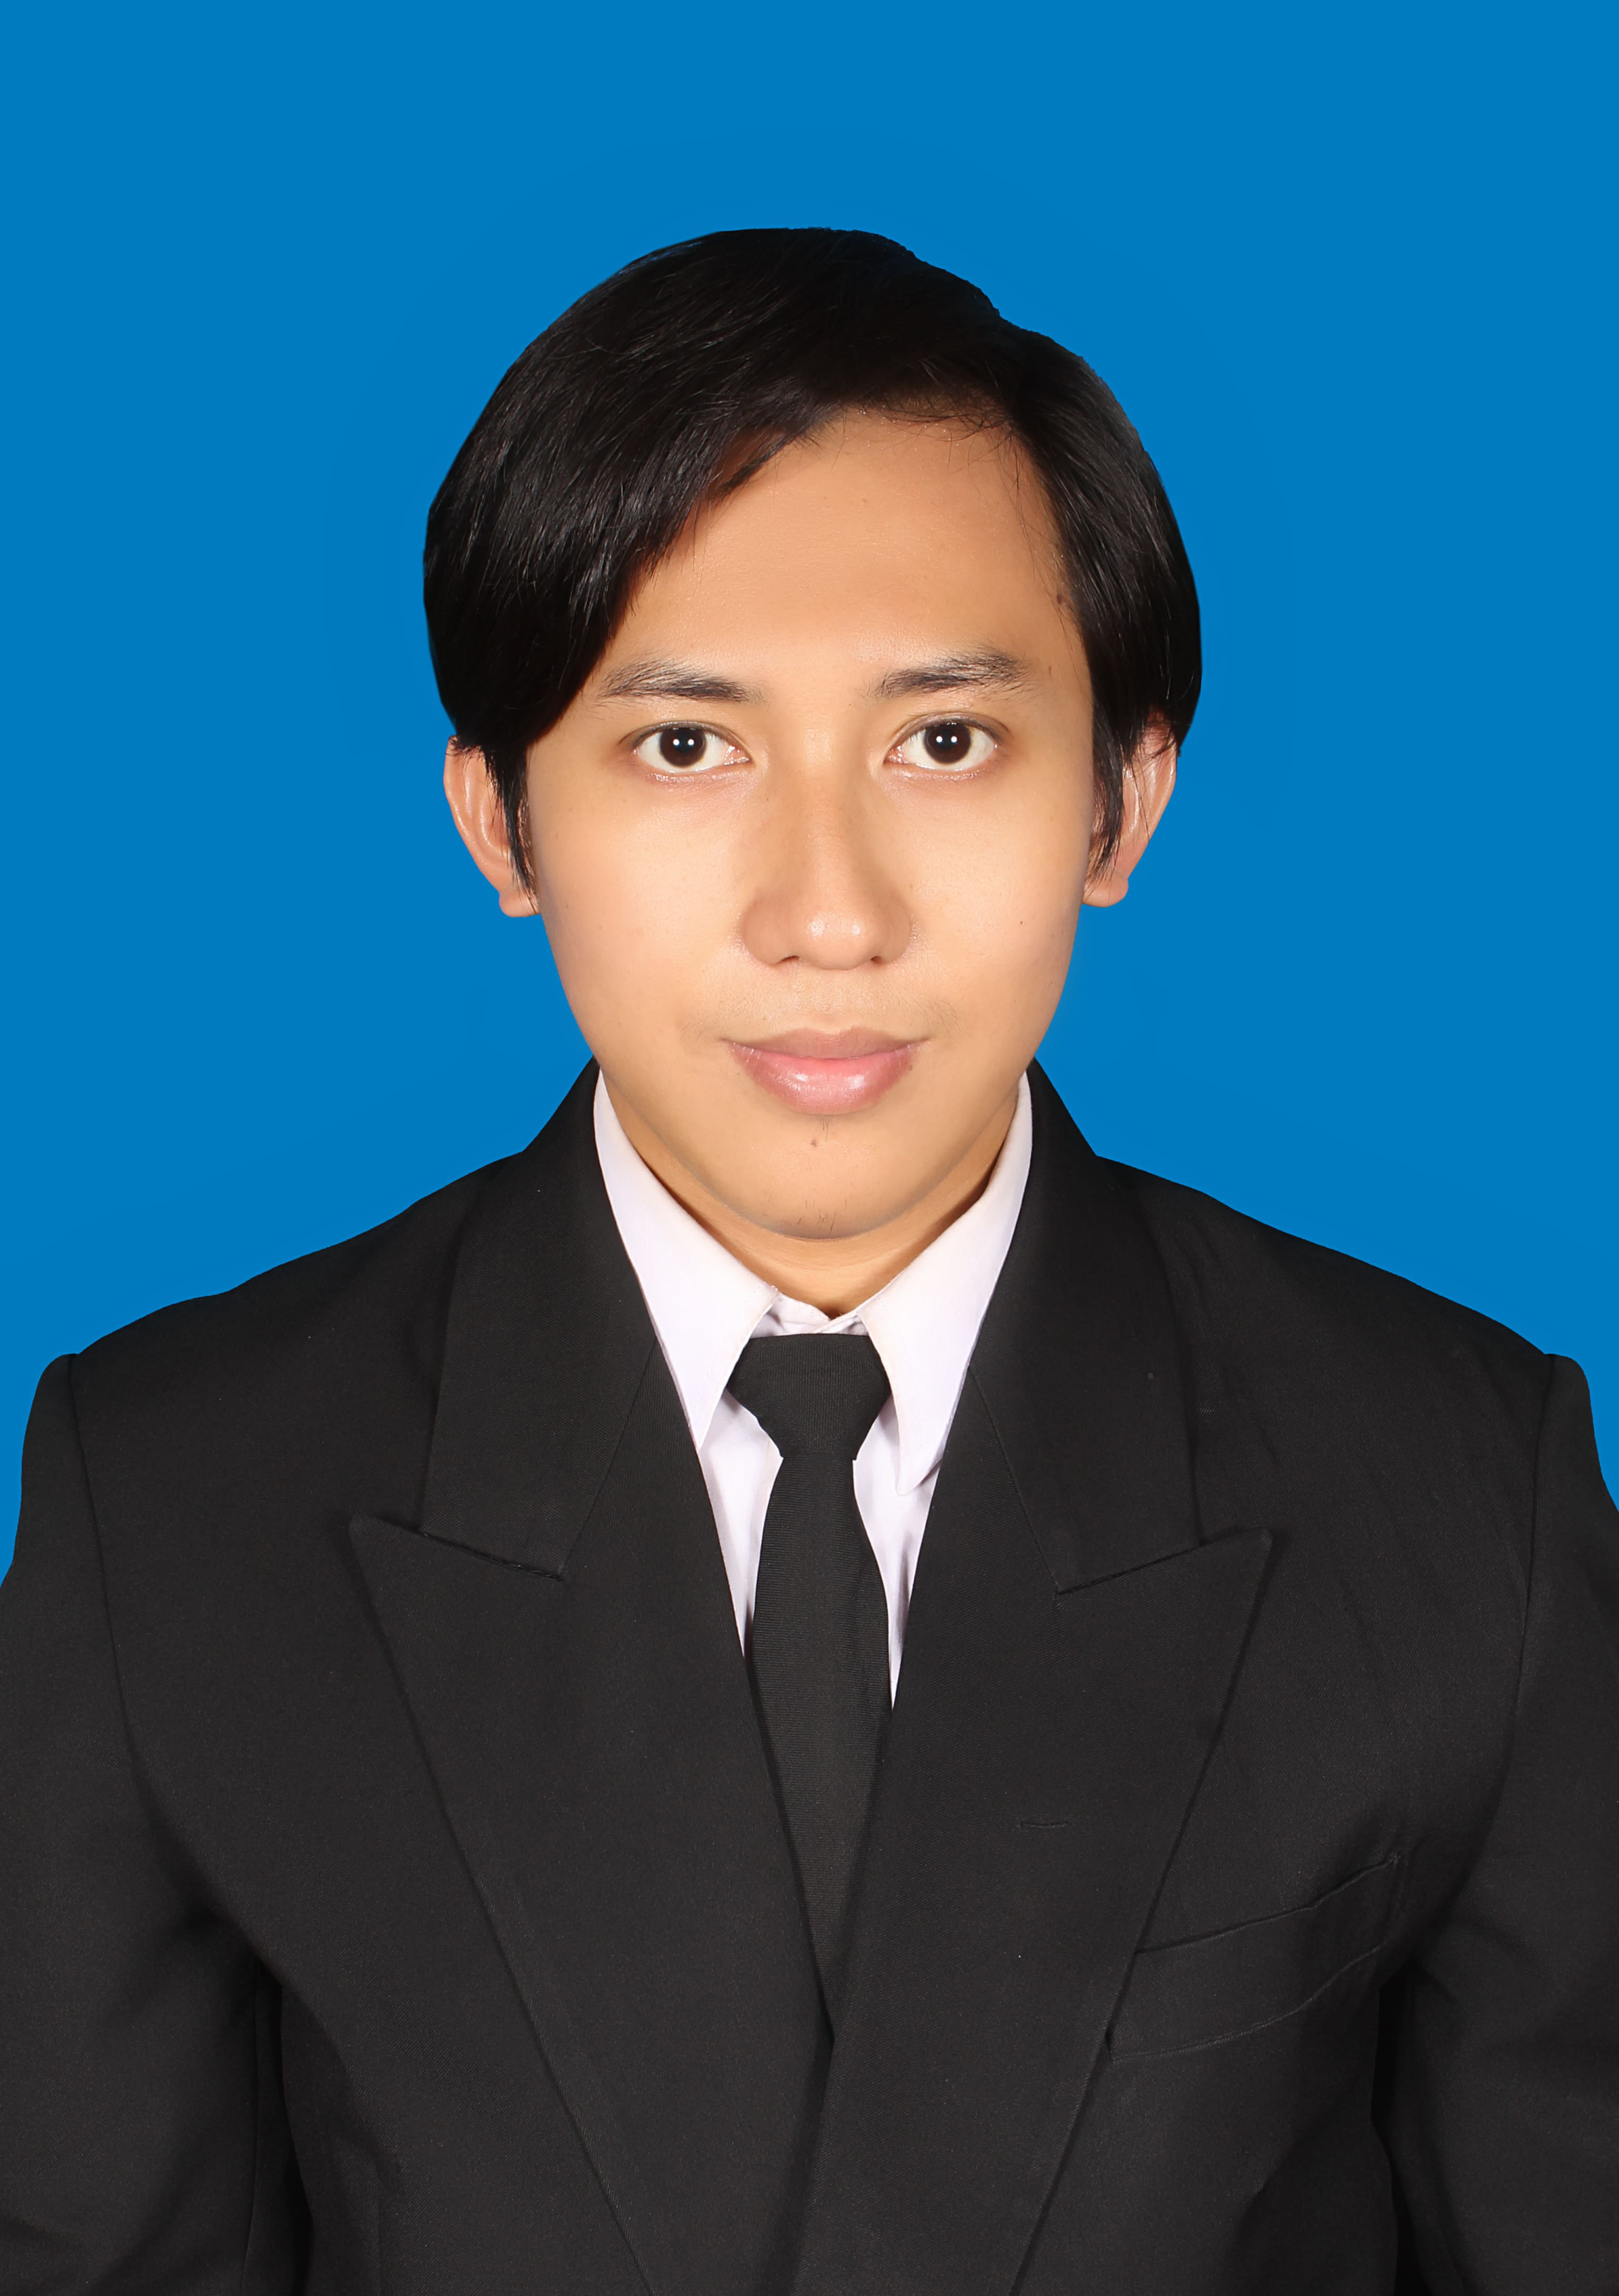
\includegraphics[height=0.2\textheight]{./ubah/foto_amik.jpg}
\end{center}
%*********************************
\section*{Personal Identity}
\begin{tabular}{p{3cm}cp{9cm}}
	%Masukan Identitas Disini.............
	Nama          & : &
	Amik Rafly Azmi Ulya                           \\
	Tempat Lahir  & : &
	Jepara                                         \\
	Tanggal Lahir & : &
	14 November 1999                               \\
	Alamat        & : &
	Mangkuyudan, Kartasura, Sukoharjo, Jawa Tengah \\
\end{tabular}

\section*{Educational Background}
\begin{tabular}{p{3cm}cp{9cm}}
	2022-2024 & : &
	Master Degree (S2), Department of Electrical Engineering, Faculty of Intelligent Electrical and Informatics Technology, Institut Teknologi Sepuluh Nopember \\
	          &   &                                                                                                                                             \\
	2018-2022 & : &
	Bachelor Degree (S1), Departement of Physics, Faculty of Science and Data Analytics, Institut Teknologi Sepuluh Nopember                                    \\
	          &   &                                                                                                                                             \\
	2015-2018 & : &
	2\textsuperscript{nd} Kudus Islamic State Senior High School (MAN)                                                                                          \\
	          &   &                                                                                                                                             \\
	2012-2015 & : &
	Unggulan Pondok Modern Selamat Junior High School (SMP)                                                                                                     \\
	          &   &                                                                                                                                             \\
	2006-2012 & : &
	Al-Islam Kartasura Islamic Elementary School (MI)                                                                                                           \\
\end{tabular}


\section*{Publication List}

\begin{enumerate}
	\item Amik Rafly Azmi Ulya et al. “HiroPoseEstimation: A Dataset of Pose Estimation for Kid-Size Humanoid Robot”. In: Journal of Information Technology and Computer Science 8.3 (2023), 231–240. DOI: 10.25126/ jitecs.202383568. URL: https://jitecs.ub.ac.id/index.php/ jitecs/article/view/568.
\end{enumerate}

% \section*{Riwayat Penelitian}
% \begin{enumerate}
% 	\item \lipsum[3]
% 	\item \lipsum[3]
% 	\item Penelitian Ke Tiga
% 	\item Penelitian Ke Empat
% \end{enumerate}
% \section*{Riwayat Lainnya}

% \lipsum[1]